\documentclass{beamer}
\usepackage{tikz}
\usetikzlibrary{math}

\usepackage{pgfplots}
\usepgfplotslibrary{polar}

%Please read on the commands and options used below (either in the TikZ / PGFPlots manuals, or elsewhere).

\usepackage{filecontents}
% We're defining a file that will be created upon LaTeX compilation.
% Please note that you need to manually delete the file if you make changes,
% as filecontents does not overwrite files (for obvious security reasons).
\begin{filecontents*}{mpg.csv}
mpg,cylinders,displacement,horsepower,weight,acceleration,model_year,origin,name
18,8,307,130,3504,12,70,1,chevrolet chevelle malibu
15,8,350,165,3693,11.5,70,1,buick skylark 320
18,8,318,150,3436,11,70,1,plymouth satellite
16,8,304,150,3433,12,70,1,amc rebel sst
17,8,302,140,3449,10.5,70,1,ford torino
15,8,429,198,4341,10,70,1,ford galaxie 500
14,8,454,220,4354,9,70,1,chevrolet impala
14,8,440,215,4312,8.5,70,1,plymouth fury iii
14,8,455,225,4425,10,70,1,pontiac catalina
15,8,390,190,3850,8.5,70,1,amc ambassador dpl
15,8,383,170,3563,10,70,1,dodge challenger se
\end{filecontents*}

\begin{document}

\begin{frame}
  \begin{figure}
    \center
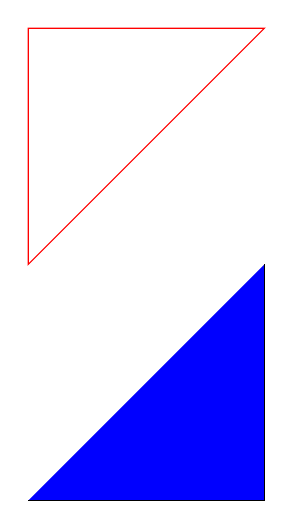
\begin{tikzpicture}[scale=3]
  \draw [fill=blue] (0, 0) -- (1, 0) -- (1, 1);
  \draw [red] (1, 2) -- (0, 2) -- (0, 1) -- cycle;
\end{tikzpicture}
    \caption{Example 1: Vector drawing in TikZ}
  \end{figure}
\end{frame}

\begin{frame}
  \begin{figure}
    \centering
    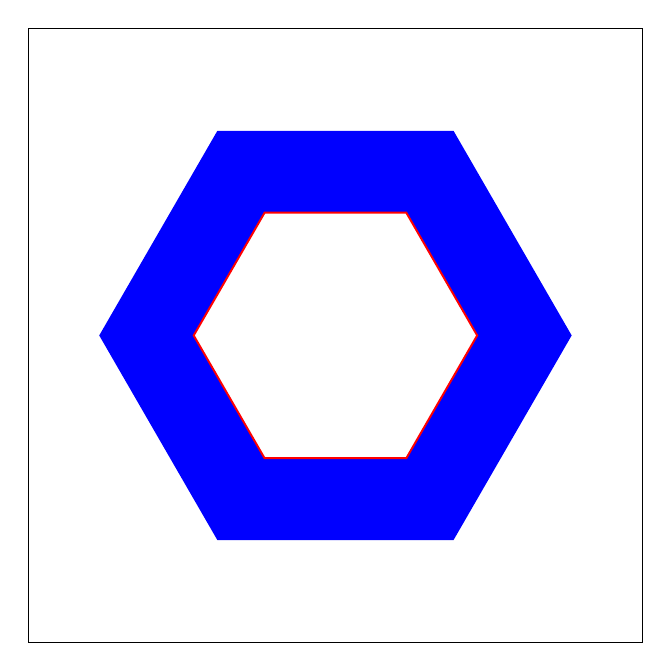
\begin{tikzpicture}[scale=3]
      \draw[line width=0.5pt, black] (-1.3,-1.3) rectangle (1.3,1.3);
      \path[fill=blue, draw=none, even odd rule]
        (0:1) -- (60:1) -- (120:1) -- (180:1) -- (240:1) -- (300:1) -- cycle
        (300:0.6) -- (240:0.6) -- (180:0.6) -- (120:0.6) -- (60:0.6) -- (0:0.6) -- cycle;
      \draw[red, line width=0.7pt]
        (0:0.6) -- (60:0.6) -- (120:0.6) --
        (180:0.6) -- (240:0.6) -- (300:0.6) -- cycle;

    \end{tikzpicture}
    \caption{Task 1: Hexagon drawing}
  \end{figure}
\end{frame}

\begin{frame}
  \begin{figure}
    \center
  \begin{tikzpicture}[scale=3]
    % Don't forget ; in \tikzmath. Even after } .
    \tikzmath{%Do not leave empty lines inside tikzmath. Use comments for visual separation
      \xmin = +1000; \xmax = -1000; \ymin = +1000; \ymax = -1000;
      % \tmin = -pi/2;
      % \tmax =  pi/2;
      % \step = 0.05;
      % tikz expects angles in degrees
      \tmin = -90; % -pi / 2 (* 360 / (2*pi))
      \tmax = 90;
      \step = 0.05 * 180 / pi;
      \a = 1;
      \b = 2;
      %{start, ...increment, end}
      for \t in {\tmin + \step, ...\step,\tmax - \step} {
        \x = \a + \b * cos(\t);
        \y = \a * tan(\t) + \b * sin(\t);
        if \x < \xmin then {
          \xmin = \x;
        };
        if \x > \xmax then {
          \xmax = \x;
        };
        if \y < \ymin then {
          \ymin = \y;
        };
        if \y > \ymax then {
          \ymax = \y;
        };
        %
        \x = \a - \b * cos(\t);
        \y = \a * tan(\t) - \b * sin(\t);
        if \x < \xmin then {
          \xmin = \x;
        };
        if \x > \xmax then {
          \xmax = \x;
        };
        if \y < \ymin then {
          \ymin = \y;
        };
        if \y > \ymax then {
          \ymax = \y;
        };
      };
      \xmax = abs(\xmax);
      \xmin = abs(\xmin);
      \ymax = abs(\ymax);
      \ymin = abs(\ymin);
      if \xmin > \xmax then {
        \xmax = \xmin;
      };
      if \ymin > \ymax then {
        \ymax = \ymin;
      };
      %
      \xmprev = (\a + \b * cos(\tmin + \step)) / \xmax;
      \ymprev = (\a * tan(\tmin + \step) + \b * sin(\tmin + \step)) / \ymax;
      for \t in {\tmin + \step, ...\step,\tmax - \step} {
        \xm = (\a + \b * cos(\t)) / \xmax;
        \ym = (\a * tan(\t) + \b * sin(\t)) / \ymax;
        {\draw[blue] (\xmprev, \ymprev) -- (\xm, \ym);};
        \xmprev = \xm;
        \ymprev = \ym;
      };
      \xmprev = (\a - \b * cos(\tmin + \step)) / \xmax;
      \ymprev = (\a * tan(\tmin + \step) - \b * sin(\tmin + \step)) / \ymax;
      for \t in {\tmin + \step, ...\step,\tmax - \step} {
        \xm = (\a - \b * cos(\t)) / \xmax;
        \ym = (\a * tan(\t) - \b * sin(\t)) / \ymax;
        {\draw[blue] (\xmprev, \ymprev) -- (\xm, \ym);};
        \xmprev = \xm;
        \ymprev = \ym;
      };
    }
  \end{tikzpicture}
  \caption{Example 2.1: Nicomedes' Conchoid}
\end{figure}
\end{frame}

\begin{frame}
  \begin{figure}
    \center
  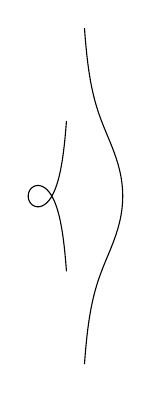
\begin{tikzpicture}
    \def\a{1}
    \def\b{2}
    % {-90+1} so we don't divide by 0. The other +10 are so that we
    % get the picture we want. See the next tikzpicture for a (worse) variant.
    \draw[scale=0.3,domain={-90+11}:{90-11},smooth,variable=\t,samples=180] plot ({\a + \b * cos(\t)}, {\a * tan(\t) + \b * sin(\t)});
    \draw[scale=0.3,domain={-90+11}:{90-11},smooth,variable=\t,samples=180] plot ({\a - \b * cos(\t)}, {\a * tan(\t) - \b * sin(\t)});
  \end{tikzpicture} \hfill
  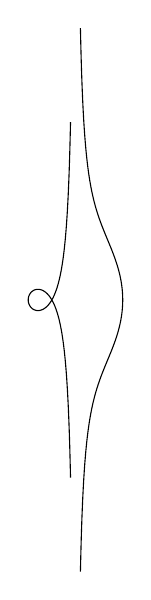
\begin{tikzpicture}
    \def\a{1}
    \def\b{2}
    \draw[scale=0.3,domain={-90+6}:{90-6},smooth,variable=\t,samples=180] plot ({\a + \b * cos(\t)}, {\a * tan(\t) + \b * sin(\t)});
    \draw[scale=0.3,domain={-90+6}:{90-6},smooth,variable=\t,samples=180] plot ({\a - \b * cos(\t)}, {\a * tan(\t) - \b * sin(\t)});
  \end{tikzpicture}
  \caption{Example 2.2: Nicomedes' Conchoid, auto-plot}
\end{figure}
\end{frame}


\begin{frame}
  \begin{figure}
    \center
    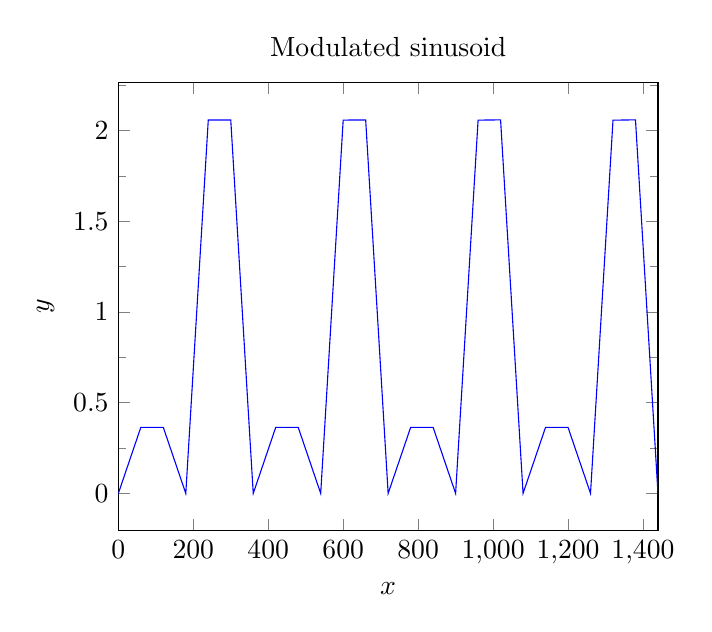
\begin{tikzpicture}
      \begin{axis}[
        title=Modulated sinusoid,
        xlabel={$x$},
        ylabel={$y$},
        domain={0}:{8 * 180}, %8 * pi
        xmin=0, xmax= {8 * 180}, %the actual limits of the plot
        minor y tick num=1, %how many unlabeled ticks between labeled ticks
        ]
        \addplot [blue] {abs(sin(x)) * exp(-sin(x))};
    \end{axis} 
    \end{tikzpicture}
    \caption{Example 2.3: Modulated sinusoid, using PGFPlots. Rough.}
  \end{figure}
\end{frame}

\begin{frame}
  \begin{figure}
    \center
    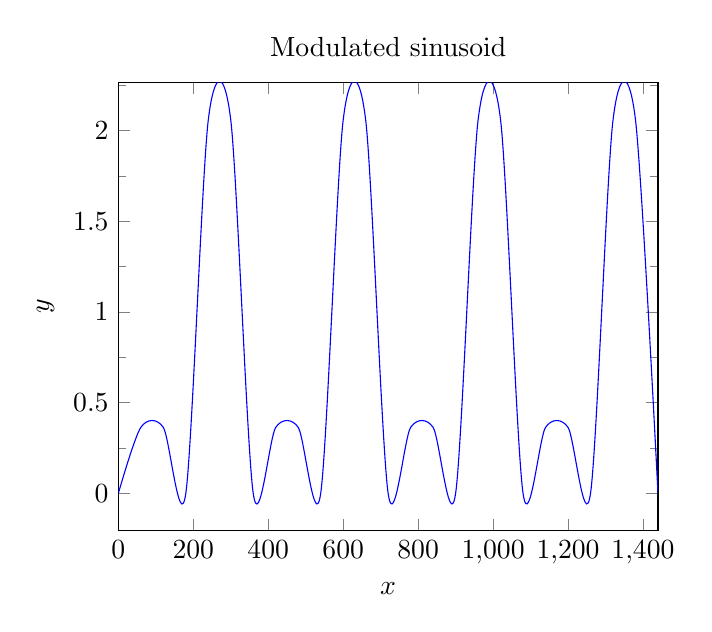
\begin{tikzpicture}
      \begin{axis}[
        title=Modulated sinusoid,
        xlabel={$x$},
        ylabel={$y$},
        domain={0}:{8 * 180}, %8 * pi
        xmin=0, xmax= {8 * 180}, %the actual limits of the plot
        minor y tick num=1, %how many unlabeled ticks between labeled ticks
        smooth,
        ]
        \addplot [blue] {abs(sin(x)) * exp(-sin(x))};
    \end{axis} 
    \end{tikzpicture}
    \caption{Example 2.4: Modulated sinusoid, using PGFPlots. Rough, artificially smoothed.}
  \end{figure}
\end{frame}

\begin{frame}
  \begin{figure}
    \center
    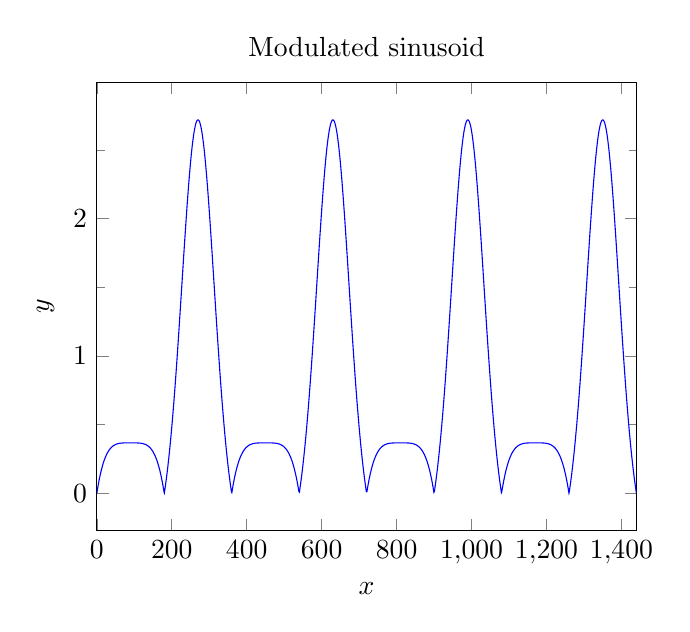
\begin{tikzpicture}
      \begin{axis}[
        title=Modulated sinusoid,
        xlabel={$x$},
        ylabel={$y$},
        domain={0}:{8 * 180}, %8 * pi
        xmin=0, xmax= {8 * 180}, %the actual limits of the plot
        minor y tick num=1, %how many unlabeled ticks between labeled ticks
        smooth,
        samples=1000,
        ]
        \addplot [blue] {abs(sin(x)) * exp(-sin(x))};
    \end{axis} 
    \end{tikzpicture}
    \caption{Example 2.5: Modulated sinusoid, using PGFPlots. Better sampled.}
  \end{figure}
\end{frame}

\begin{frame}
  \begin{figure}
    \centering
    \begin{tikzpicture}[scale=2]
      % Circle Concoid (forma tip limaçon):
      \draw[domain=0:360, samples=400, smooth, variable=\t]
        plot ({(1 + 2*cos(\t)) * cos(\t)},
              {(1 + 2*cos(\t)) * sin(\t)});
    \end{tikzpicture}
    \caption{Task 2: Circle Concoid}
  \end{figure}
\end{frame}



\begin{frame}
\begin{figure}
  \center
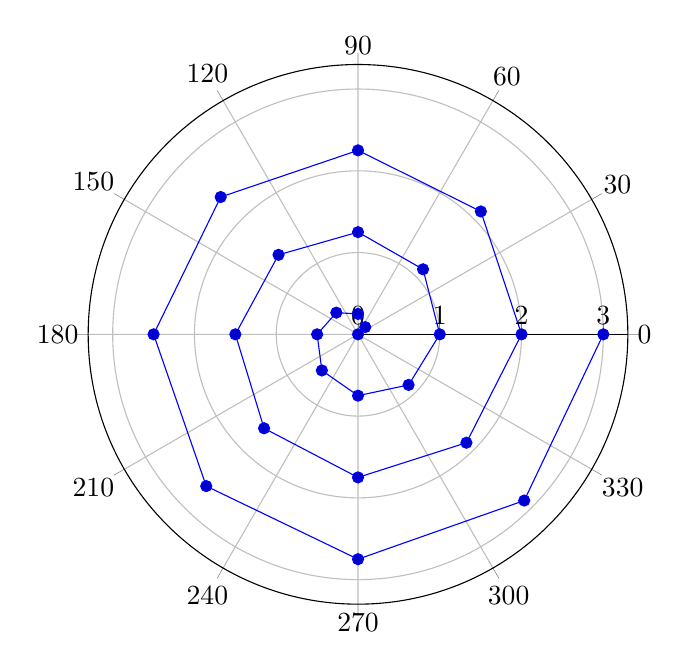
\begin{tikzpicture}
  \begin{polaraxis}
    %try \addplot, notice the difference
    \addplot+ [domain=0:3] (360*x,x); % (angle,radius)
\end{polaraxis} 
\end{tikzpicture}
  \caption{Example 3: Polar plotting}
\end{figure}
\end{frame}

\begin{frame}
  \begin{figure}
    \centering
    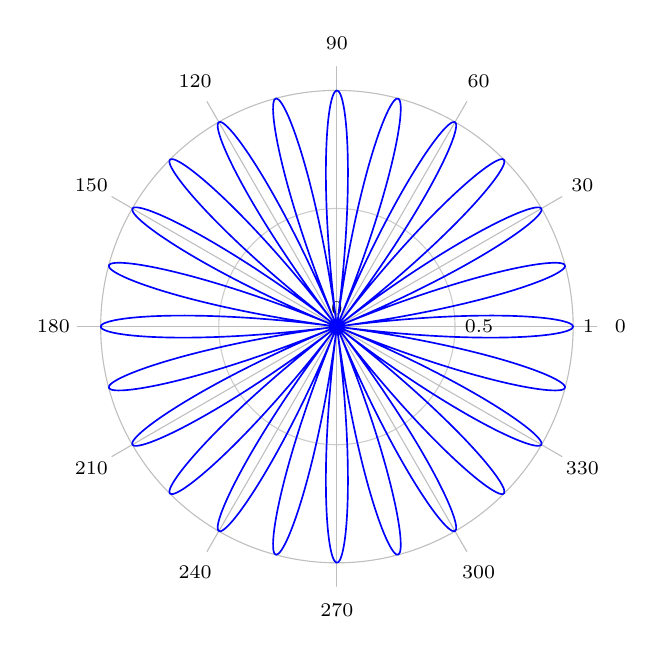
\begin{tikzpicture}[scale=3.0, line cap=round, line join=round]
      
      % --- CERCURI CONCENTRICE ---
      \draw[thin, gray!50] (0,0) circle (1);   % cerc exterior
      \draw[thin, gray!40] (0,0) circle (0.5); % cerc intermediar (raza 0.5)
      
      % --- LINII RADIALE SI ETICHETE UNGHI ---
      \foreach \ang in {0,30,...,330} {
        \draw[thin, gray!50] (0,0) -- (\ang:1.1);
        \node[font=\scriptsize] at (\ang:1.2) {\ang};
      }
      
      % --- ETICHETE PENTRU RAZELE ---
      \node[font=\scriptsize, anchor=west] at (0:0.5) {0.5};
      \node[font=\scriptsize, anchor=west] at (0:1)   {1};
      
      % --- AFISAREA LUI "0" IN CENTRU ---
      \node[font=\scriptsize, anchor=south, yshift=1pt] at (0,0) {0};

      
      % --- CURBA (r = cos(12·θ)) = "Rose curve" ---
      \draw[blue, line width=0.6pt, domain=0:360, samples=720, smooth, variable=\t]
        plot ({cos(12*\t)*cos(\t)}, {cos(12*\t)*sin(\t)});
      
    \end{tikzpicture}
    \caption{Task 3: Polar plotting}
  \end{figure}
\end{frame}

\begin{frame}
  \begin{figure}
    \center
    \begin{tikzpicture}
      \begin{axis} [
        title=Miles per gallon,
        xlabel=hosepower,
        ylabel=mpg,
        ]
        \addplot coordinates {
          (140, 18)
          (140, 17)
          (150, 16)
          (180, 15)
          (220, 14)
        };
        %try removing only marks
        \addplot table [x=horsepower, y=mpg, col sep=comma, only marks] {mpg.csv};
    \end{axis} 
    \end{tikzpicture}
    \caption{Example 4: Plotting datafiles, and coordinates.}
  \end{figure}
\end{frame}

\begin{filecontents}{mydata.dat}
horsepower   mpg
40   42
45   44
50   41
60   40
70   38
80   35
90   33
100  28
110  29
120  26
130  23
140  22
150  21
160  20
170  18
180  17
190  16
200  15
210  14
\end{filecontents}



\begin{tikzpicture}
    \begin{axis}[
        title={Miles per gallon},       % Titlul graficului
        xlabel={horsepower},            % Eticheta axei X
        ylabel={mpg},                   % Eticheta axei Y
        xmin=40, xmax=240,              % Limite axa X (ajustate usor)
        ymin=5, ymax=50,                % Limite axa Y
        xtick={50, 100, 150, 200},      % Marcaje pe axa X
        ytick={10, 20, 30, 40, 50},      % Marcaje pe axa Y
        legend pos=north west,          % Pozitia legendei (daca e necesara)
        grid=major,                     % Grila principala (optional, nu era in imagine)
        grid style={dashed, gray!30},   % Stilul grilei (optional)
        width=10cm,                     % Latimea graficului
        height=8cm,                     % Inaltimea graficului
        scatter/classes={               % Definire clasa pentru scatter plot
            a={mark=*, blue}            % Puncte albastre
        }
    ]

    % Plotarea datelor din fisier (scatter plot)
    % Asigura-te ca fisierul 'auto_data.dat' exista in acelasi director
    % si are coloanele 'hp' si 'mpg'
    \addplot [
        scatter, only marks,            % Tip grafic: scatter, doar marcaje
        scatter src=explicit symbolic   % Sursa pentru stilul marcajelor
    ]
    table [x=hp, y=mpg, meta=label] {
        hp mpg label
        % Aici ar trebui sa fie datele din fisierul auto_data.dat
        % Am pus cateva puncte direct pentru exemplu, dar ideal e sa citesti fisierul
        % Inlocuieste liniile de mai jos cu: table [x=hp, y=mpg, meta expr={"a"}] {auto_data.dat};
         70 35 a
         80 32 a
         90 28 a
        100 25 a
        110 23 a
        120 21 a
        130 20 a
        140 18 a
        150 17 a
        160 16 a
        170 15 a
        180 14 a
        190 13 a
        200 12 a
        210 11 a
         50 45 a
         60 42 a
         75 38 a
         85 34 a
         95 30 a
        105 27 a
        115 24 a
        125 22 a
        135 19 a
        145 18 a
        155 17 a
        165 16 a
        175 15 a
        185 14 a
        195 13.5 a
        205 12.5 a
        215 11.5 a
        225 11 a
         55 44 a
         65 40 a
         88 31 a
        112 26 a
        133 21 a
        158 17.5 a
        188 14.5 a
        208 12.8 a
    };
    % Nota: Folosirea tabelului inline este doar demonstrativa.
    % Metoda corecta:
    \addplot [scatter, only marks, scatter src=explicit symbolic]
    table [x=hp, y=mpg, meta expr={"a"}] {auto_data.dat};

    % Plotarea functiei polinomiale (regresie)
    % Aceasta este o aproximare a curbei din imagine.
    % Coeficientii reali ar trebui obtinuti din regresia facuta in R.
    \addplot [
        domain=50:230,      % Domeniul pe axa X pentru care se traseaza functia
        samples=100,        % Numarul de puncte pentru a trasa curba lin
        color=red,          % Culoarea liniei
        thick               % Grosimea liniei (optional)
    ]
    {0.0005*x^2 - 0.25*x + 50}; % Functia polinomiala aproximativa

    \end{axis}
\end{tikzpicture}

% Adaugarea figurii si a caption-ului intr-un document standard (ex: article)
% Daca folosesti clasa standalone, aceasta parte nu este necesara direct in acelasi fisier.
% \documentclass{article}
% \usepackage{pgfplots}
% \usepackage{amsmath}
% \pgfplotsset{compat=1.18}
% \usepackage{graphicx} % Necesar pentru \captionof daca nu e in float
% \usepackage{caption}  % Pentru \captionof
%
% \begin{document}
% ... text ...
%
% \begin{figure}[htbp] % h=here, t=top, b=bottom, p=page of floats
%     \centering
%     % Include aici codul TikZ/pgfplots de mai sus
%     \begin{tikzpicture}
%         \begin{axis}[...]
%         ... continutul axis ...
%         \end{axis}
%     \end{tikzpicture}
%     \caption{Plotting datafiles. Make sure to clean data, and regress it externally. Here, a 2\textsuperscript{nd} degree polynomial function was fitted in R.}
%     \label{fig:mpg_vs_hp}
% \end{figure}


\end{document}
